\documentclass[t]{beamer}
\usepackage[T1]{fontenc}
%\usepackage[utf8]{inputenc}
\usepackage{lmodern}
\usepackage{amsmath}
\usepackage{amsfonts}
\usepackage{amssymb}
\usepackage{amsthm}
\usepackage{graphicx}
\usepackage{color}
\usepackage{xcolor}
\usepackage{url}
\usepackage{textcomp}
\usepackage{listings}
\usepackage{hyperref}
\usepackage{parskip}
\usetheme{default}
\usepackage{minted}
\usepackage{multicol}
\usepackage{animate}
\usepackage{multimedia}

\usetheme[progressbar=frametitle]{metropolis}
\setbeamertemplate{frame numbering}[fraction]
\definecolor{vala}{rgb}{.482,.424,.639}
\definecolor{valadark}{rgb}{.241,.212,.320}
\setbeamercolor*{structure}{bg=vala!20,fg=vala}

\setbeamercolor*{palette primary}{use=structure,fg=white,bg=structure.fg}
\setbeamercolor*{palette secondary}{use=structure,fg=white,bg=structure.fg!75}
\setbeamercolor*{palette tertiary}{use=structure,fg=white,bg=structure.fg!50!black}
\setbeamercolor*{palette quaternary}{fg=white,bg=black}

\setbeamercolor{section in toc}{fg=black,bg=white}
%\setbeamercolor{alerted text}{use=structure,fg=structure.fg!50!black!80!black}

\setbeamercolor{titlelike}{parent=palette primary,fg=structure.fg!50!black}
\setbeamercolor{frametitle}{bg=vala!20!white,fg=vala!70!black}

%\setbeamercolor*{titlelike}{parent=palette primary}

\setbeamerfont{subsection in toc}{size=\small}

\hypersetup{
    colorlinks=true,
    linkcolor=valadark,
    citecolor=valadark,
    filecolor=valadark,
    urlcolor=vala
}

\newcommand{\fancyurl}[1]{\href{#1}{#1}}

\newminted{json}{fontsize=\scriptsize, 
                   linenos,
                   numbersep=8pt,
                   gobble=4,
                   frame=lines,
                   bgcolor=bg,
                   framesep=3mm}

\title{Improving the Vala developer experience}
\author{Princeton Ferro}
\date{July 22, 2022}

\begin{document}

\setbeamertemplate{caption}{\raggedright\insertcaption\par}

% Goals:
% - Respond to ebassi's blog post
% - Inspire contributors to Vala
% - Show improvements to Vala
% - Philosophize about how to build a successful language
% - Establish reasonable expectations for Vala
% - Explain plans for Vala

% Outline:
% 1. Improvements to tooling:
%  - Vala Language Server (& History)
%  - Editor support: plugins (vim, nvim, builder, vscode)
%  - Project templates (valdo)
% 2. Vala community improvements:
%  - Discord
%  - Twitter
%  - GitHub organization / consolidation of Vala projects
%  - New website (vala.dev)
%  - Documentation (in progress - gitlab.gnome.org)
% 3. Plans for Vala:
%  - Static analyzer (abstract interpretation)
%  - GDB support
%  - Richer type system
%  - Code actions / linter

\begin{frame}
    \titlepage
\end{frame}

\begin{frame}[c]{What is Vala}
A high-level language for writing apps for the Linux desktop

Vala code $\rightarrow$ C $\rightarrow$ native code

Created as a GNOME project in 2006

Alternative to C, C++, and C\(\sharp\)

Selling points:
\begin{itemize}
    \item language constructs map to GLib, GObject
    \item use high-level abstractions at near-zero cost
    \item good interoperability with C
\end{itemize}
\end{frame}

\begin{frame}[c]{Who uses Vala}
elementary OS uses Vala for everything---apps, libraries, core, window manager, etc

\begin{figure}
    \begin{center}
        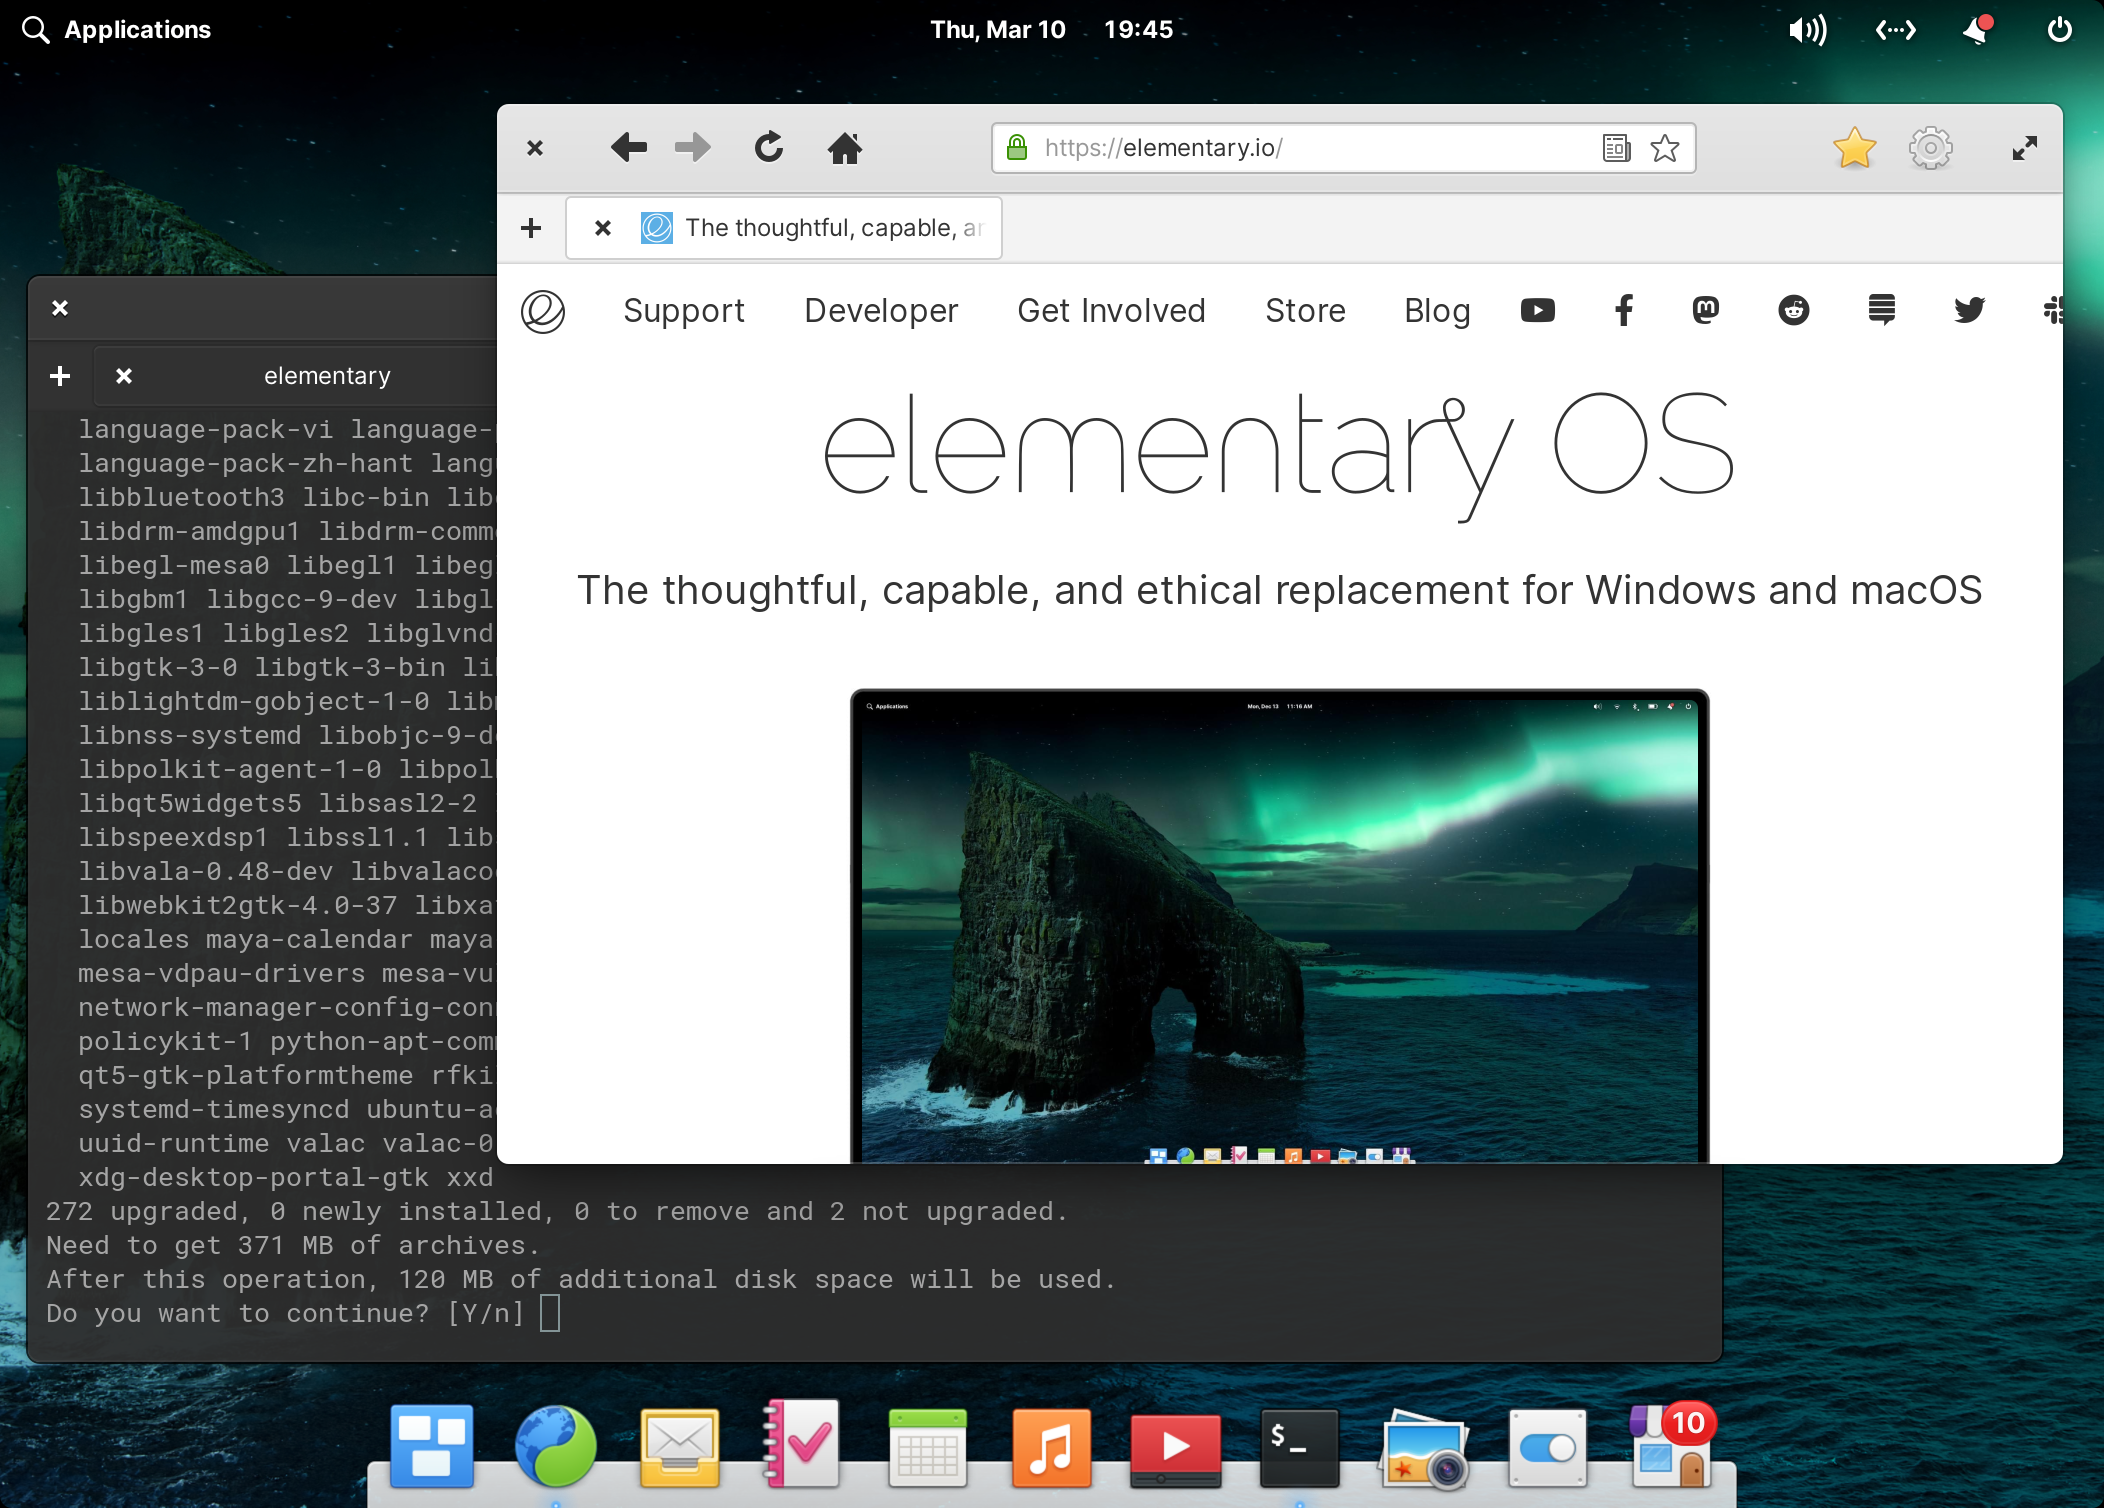
\includegraphics[scale=.125]{res/elementaryos-gala.png}
    \end{center}
\end{figure}
\end{frame}

\begin{frame}[c]{Who uses Vala}
On the GNOME side---Geary, Highscore (Games), Gitg, Boxes, Shotwell, Document Scanner

\begin{figure}
    \begin{center}
        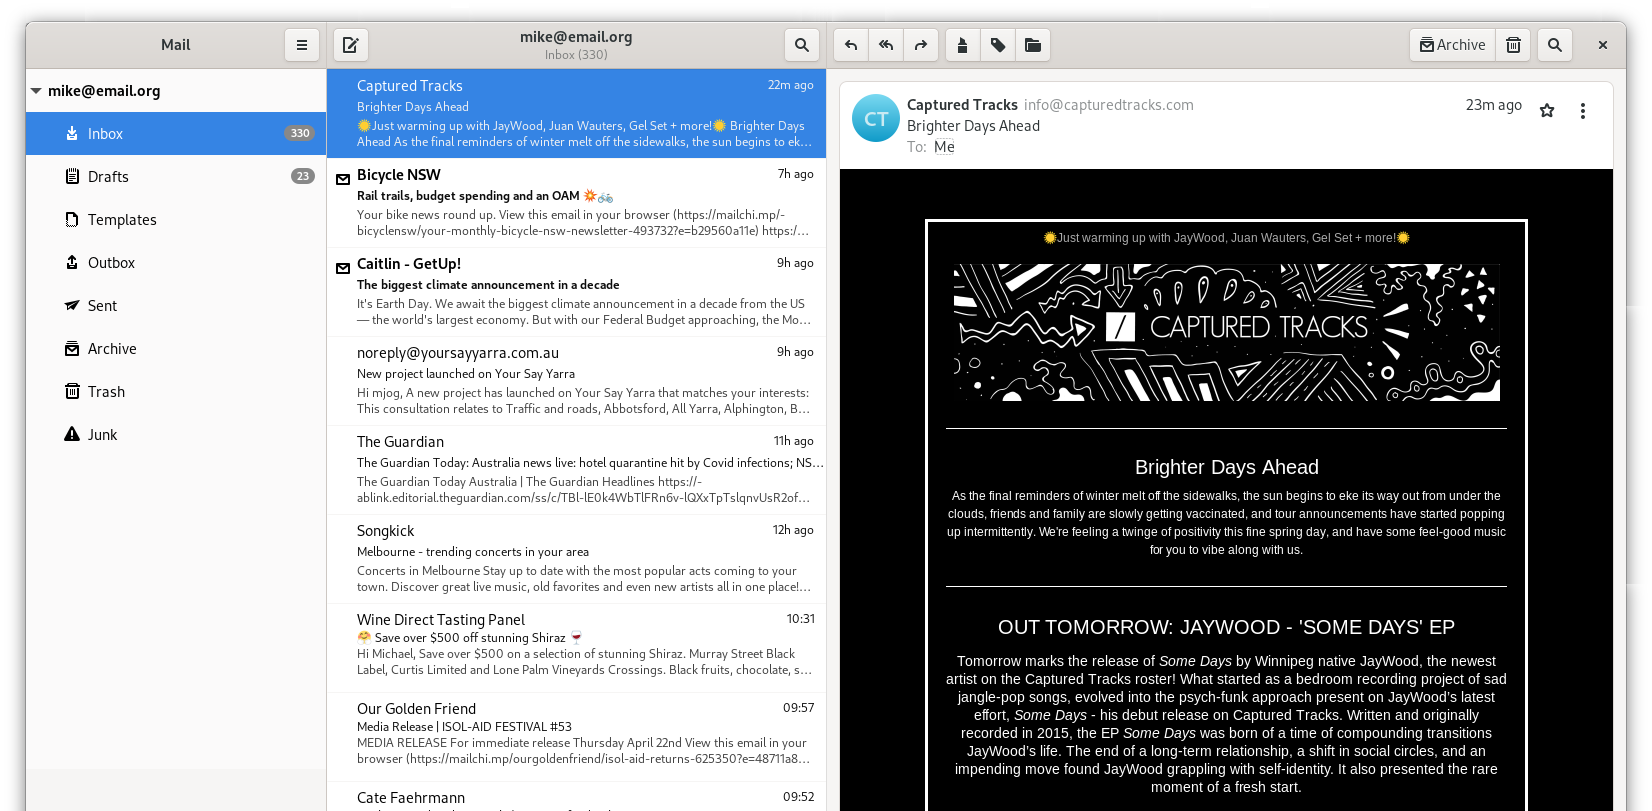
\includegraphics[scale=.18]{res/geary.png}
        \caption{Geary}
    \end{center}
\end{figure}
\end{frame}

\begin{frame}[c]{Who uses Vala}
A lot of new software created in Vala in the last five years
\begin{figure}
    \begin{center}
        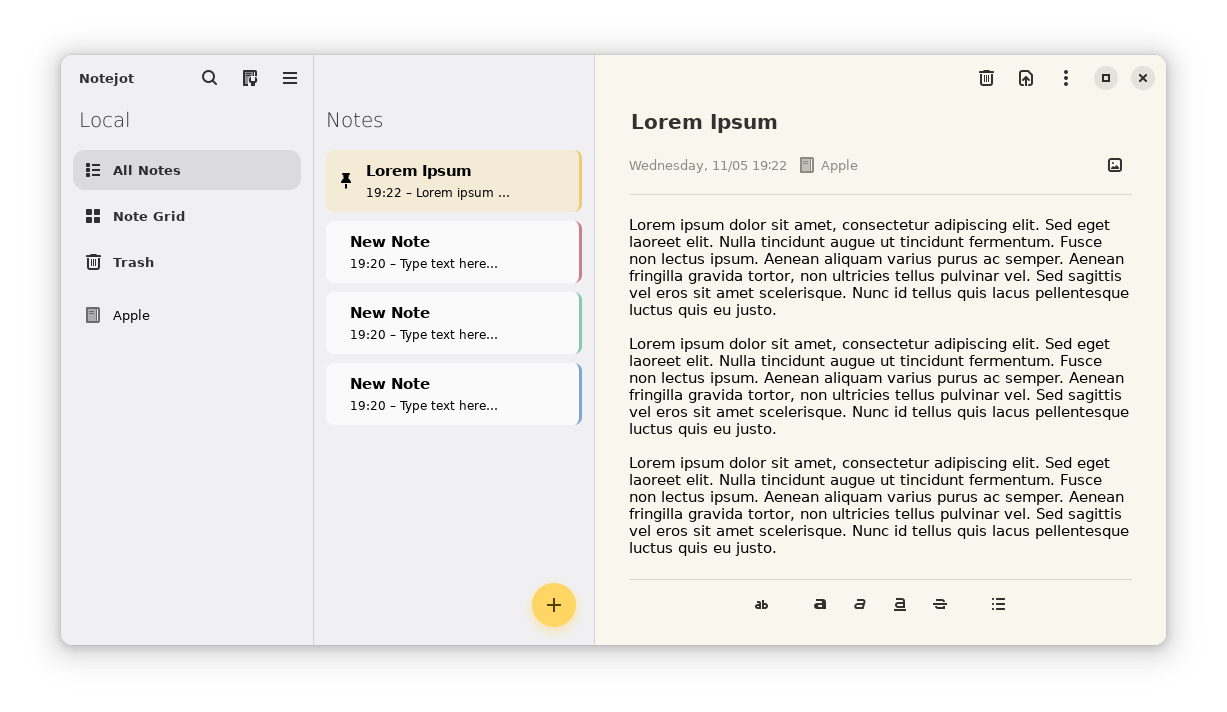
\includegraphics[scale=.23]{res/notejot.png}
        \caption{\href{https://github.com/lainsce/notejot}{Notejot by @lainsce (304 stars)}}
    \end{center}
\end{figure}
\end{frame}

\begin{frame}[c]{Who uses Vala}
\begin{figure}
    \begin{center}
        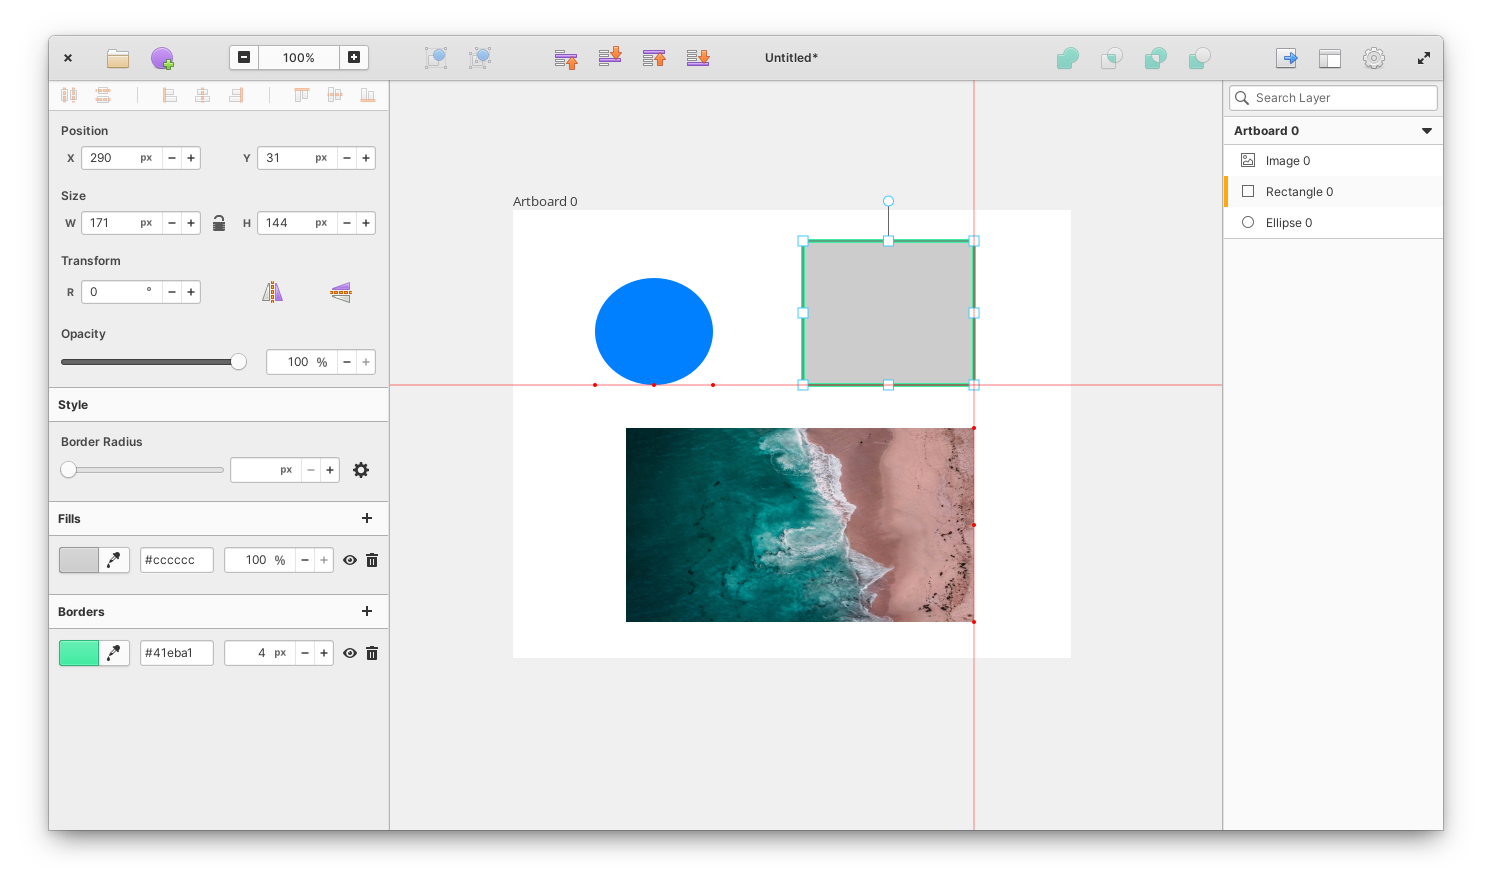
\includegraphics[scale=.205]{res/akira.png}
        \caption{\href{https://github.com/akiraux/akira}{Akira by @Alecaddd (4.8k stars)}}
    \end{center}
\end{figure}
\end{frame}

\begin{frame}[c]{Who uses Vala}
\begin{figure}
    \begin{center}
        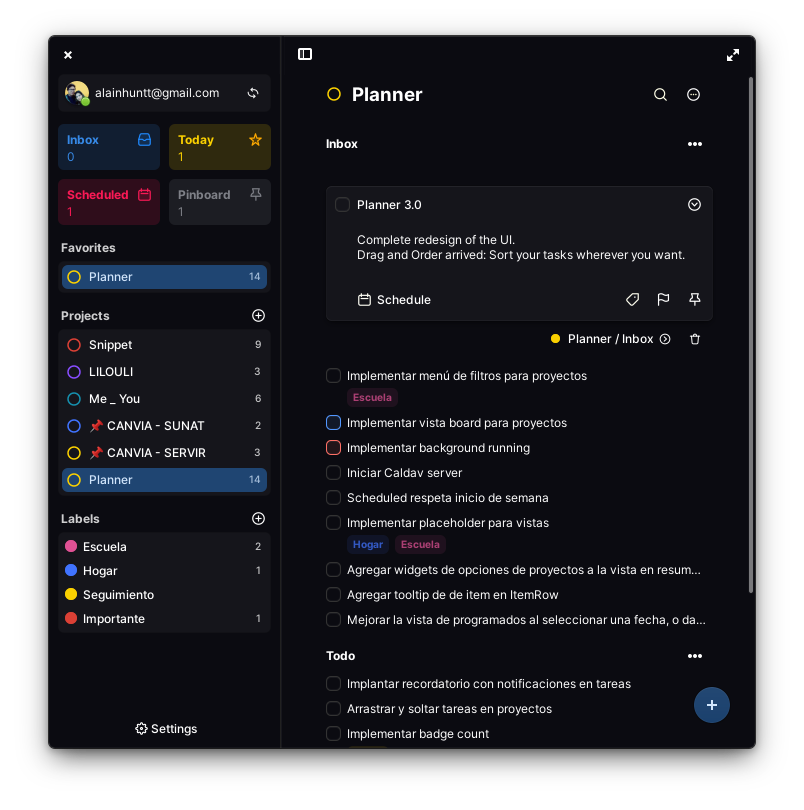
\includegraphics[scale=.25]{res/planner.png}
        \caption{\href{https://github.com/alainm23/planner}{Planner by @alainm23 (2k stars)}}
    \end{center}
\end{figure}
\end{frame}

\begin{frame}[c]{Who uses Vala}
And more:

\begin{itemize}
    \item \href{https://github.com/dino/dino}{Dino}---instant messaging (1.9k stars)
    \item \href{https://github.com/bleakgrey}{Tootle by @bleakgrey}---Mastodon client (390 stars)
    \item \href{https://github.com/IBBoard/cawbird}{Cawbird by @IBBoard}---Twitter client (301 stars)
    \item \href{https://github.com/stsdc/monitor}{Monitor by @stsdc}---system monitor (249 stars)
\end{itemize}
\end{frame}

\begin{frame}[c]{Motivation}
Vala is still used by a lot of software and new software continues to be written in Vala.

Therefore, we should improve the experience of developing software in Vala.

Make developers' lives easier---the first step to building a healthy ecosystem. \pause

Discuss recent improvements to Vala development
% Motivation for this talk and the work we're doing
% "Vala is still used by a lot of software, and a lot of new software is being written
% in it. We want to improve the experience of writing software in Vala so that it's
% up to par with the experience of writing software in languages like Rust and C#."
\end{frame}

\begin{frame}[c]{Outline}
% Outline of the rest of the talk:
%   Tooling
%   Community
%   Future plans
\vspace{12pt}
\tableofcontents
\end{frame}

\section{Tooling}
\subsection{Language server}
% What is the LSP
% Why we need a language server
% Vala Language Server:
%  - History
%  - Features
\begin{frame}[c]{Why we need a language server}
Provides online code intelligence---developers can iterate on design quickly

Provides refactoring services

Can integrate with a linter

A good language server makes a language attractive to use---Rust is supported by \texttt{rust-analyzer} and C$\sharp$ by \texttt{omnisharp-roslyn}
\end{frame}

\begin{frame}[c]{Language Server Protocol}
Simplifies writing plugins for your language of choice in \texttt{\$YOUR\_FAVORITE\_EDITOR}

Code intelligence can go into the server while clients (editors) can have a simple plugin to talk to the server.

In some cases no plugin is needed, just a few extra lines of config.
\end{frame}

\begin{frame}[c]{Vala Language Server}
Work on a language server for Vala started in 2017

Development has been slow and steady in-between sprints---a lot of work done in last two years

The language server supports many features of the LSP

Still rough around the edges

{\small Development: \url{https://github.com/vala-lang/vala-language-server}}
\end{frame}

\begin{frame}[c]{Language server features}
Support for the LSP is on par with Rust Analyzer, Clangd, and Omnisharp:
\begin{itemize}
    \item Completion
    \item Signature help
    \item Documentation on hover
    \item Code formatting
    \item Show hierarchy (calls, types)
    \item Inlay hints
    \item Refactoring (code actions, rename symbol)
    \item Code lenses (method overrides)
\end{itemize}
\end{frame}

\subsection{Editor support}
% Support across various editors
% - Vim (coc.nvim, vim-lsp)
% - Neovim (nvim-lspconfig)
% - Kate (lsp config)
% - Emacs (lsp mode)
% - Sublime Text (lsp)
% - GNOME Builder (Vala plugin)
% - Visual Studio Code (Vala plugin)
% - Tree Sitter (neovim & others)
\begin{frame}[c]{Editor support}
A variety of editors now support Vala fully (syntax highlighting + code intelligence):
\begin{itemize}
    \item Vim
    \item Neovim
    \item Kate
    \item Emacs
    \item Sublime Text
    \item GNOME Builder
    \item Visual Studio Code
\end{itemize}
\end{frame}

\begin{frame}[c]{Editor support}
    Visual Studio Code
    \begin{itemize}
        \item Install \href{https://marketplace.visualstudio.com/items?itemName=prince781.vala}{Vala plugin}
        \item Currently over 12k installs
    \end{itemize}
    
    GNOME Builder
    \begin{itemize}
        \item Bundled with VLS
        \item Enable "Vala Language Server" and disable "GVLS"
    \end{itemize}
\end{frame}

\defverbatim[colored]\exampleCode{
\begin{jsoncode}
        "languageserver": {
            "vala": {
                "command": "vala-language-server",
                "filetypes": ["vala", "genie"]
            }
        }
\end{jsoncode}
}

\begin{frame}[c]{Editor support}
    vim8/neovim
    \begin{itemize}
        \item Install \href{https://github.com/neoclide/coc.nvim}{coc.nvim}
        \item Add this to your config (\texttt{:CocConfig})
        \item Works well with \href{https://github.com/liuchengxu/vista.vim}{vista.vim} plugin.
    \end{itemize}
    \exampleCode
    
    Or you can install \href{https://github.com/neovim/nvim-lspconfig/blob/f81570d1288fd974098e0f311f728469ca919155/lua/lspconfig/vala\_ls.lua}{nvim-lspconfig} for neovim.
\end{frame}

\begin{frame}[c]{Editor support}
    Kate
    \begin{itemize}
        \item Enable built-in LSP plugin
    \end{itemize}
    
    Emacs
    \begin{itemize}
        \item Install \href{https://emacs-lsp.github.io/lsp-mode/page/lsp-vala/}{lsp-mode}
    \end{itemize}
\end{frame}

\defverbatim[colored]\exampleCode{
\begin{jsoncode}
        "clients": {
            "vala-language-server": {
                "command": [
                    "/usr/bin/vala-language-server"
                ],
                "selector": "source.vala | source.genie"
            },
        }
\end{jsoncode}
}

\begin{frame}[c]{Editor support}
    Sublime Text
    \begin{itemize}
        \item Install the \href{https://packagecontrol.io/packages/Vala-TMBundle}{Vala-TMBundle} and \href{https://github.com/sublimelsp/LSP}{LSP} packages
        \item Add config below to \texttt{LSP.sublime-settings}
        \item \texttt{Tools > LSP > Enable Language Server Globally... > vala-language-server}
    \end{itemize}
    \exampleCode
\end{frame}

\begin{frame}[c]{Editor support - Tree sitter}
Like LSP, Tree Sitter promises to be a standard way for editors to support languages.

TS API: built-in syntax highlighting and folding, easy to query document structure with grammar

{\small Grammar and highlight spec for Vala: \url{https://github.com/vala-lang/tree-sitter-vala}}

This is currently used by \href{https://github.com/nvim-treesitter/nvim-treesitter}{nvim-treesitter}
\end{frame}

\subsection{Other tools}
\begin{frame}[c]{Other tools}
\texttt{valdo} is a tool for creating new Vala projects from templates. Inspired by C$\sharp$'s \texttt{dotnet new}.

Six community-made templates (so far). Anyone can add one by opening a PR at \url{https://github.com/vala-lang/valdo}

Examples:
\begin{itemize}
    \item \texttt{valdo new} --- creates new bare Vala project w/ Meson
    \item \texttt{valdo gnome} --- creates new GNOME 40 app
    \item \texttt{valdo eos} --- creates new elementaryOS app
\end{itemize}

% valdo walks you through the setup
\end{frame}

\section{Community}
% Twitter
% Discord
% GitHub organization / consolidation of Vala projects
% New website: vala.dev
\begin{frame}[c]{Community}
% general idea is to make it easier for people to get involved
General idea is to make it easier for people to get involved

IRC is great, but not everyone wants to use it.

Twitter---post updates on Vala

Discord---general discussion and help. (really popular, 228 members so far)

We've had a lot of success with these.
\end{frame}

\subsection{GitHub organization}
\begin{frame}[c]{GitHub organization}
Consolidate Vala critical infrastructure under \href{https://github.com/vala-lang}{@vala-lang}

Choosing a popular platform lowers the barrier to entry for new contributors

Having this in one place makes it easy to track the development of the language and tooling
\end{frame}

\subsection{New website}
\begin{frame}[c]{New website}
New website: \href{https://vala.dev}{vala.dev}

{\small (\href{https://vala-project.org}{vala-project.org} will redirect you there now)}

\begin{figure}
    \begin{center}
        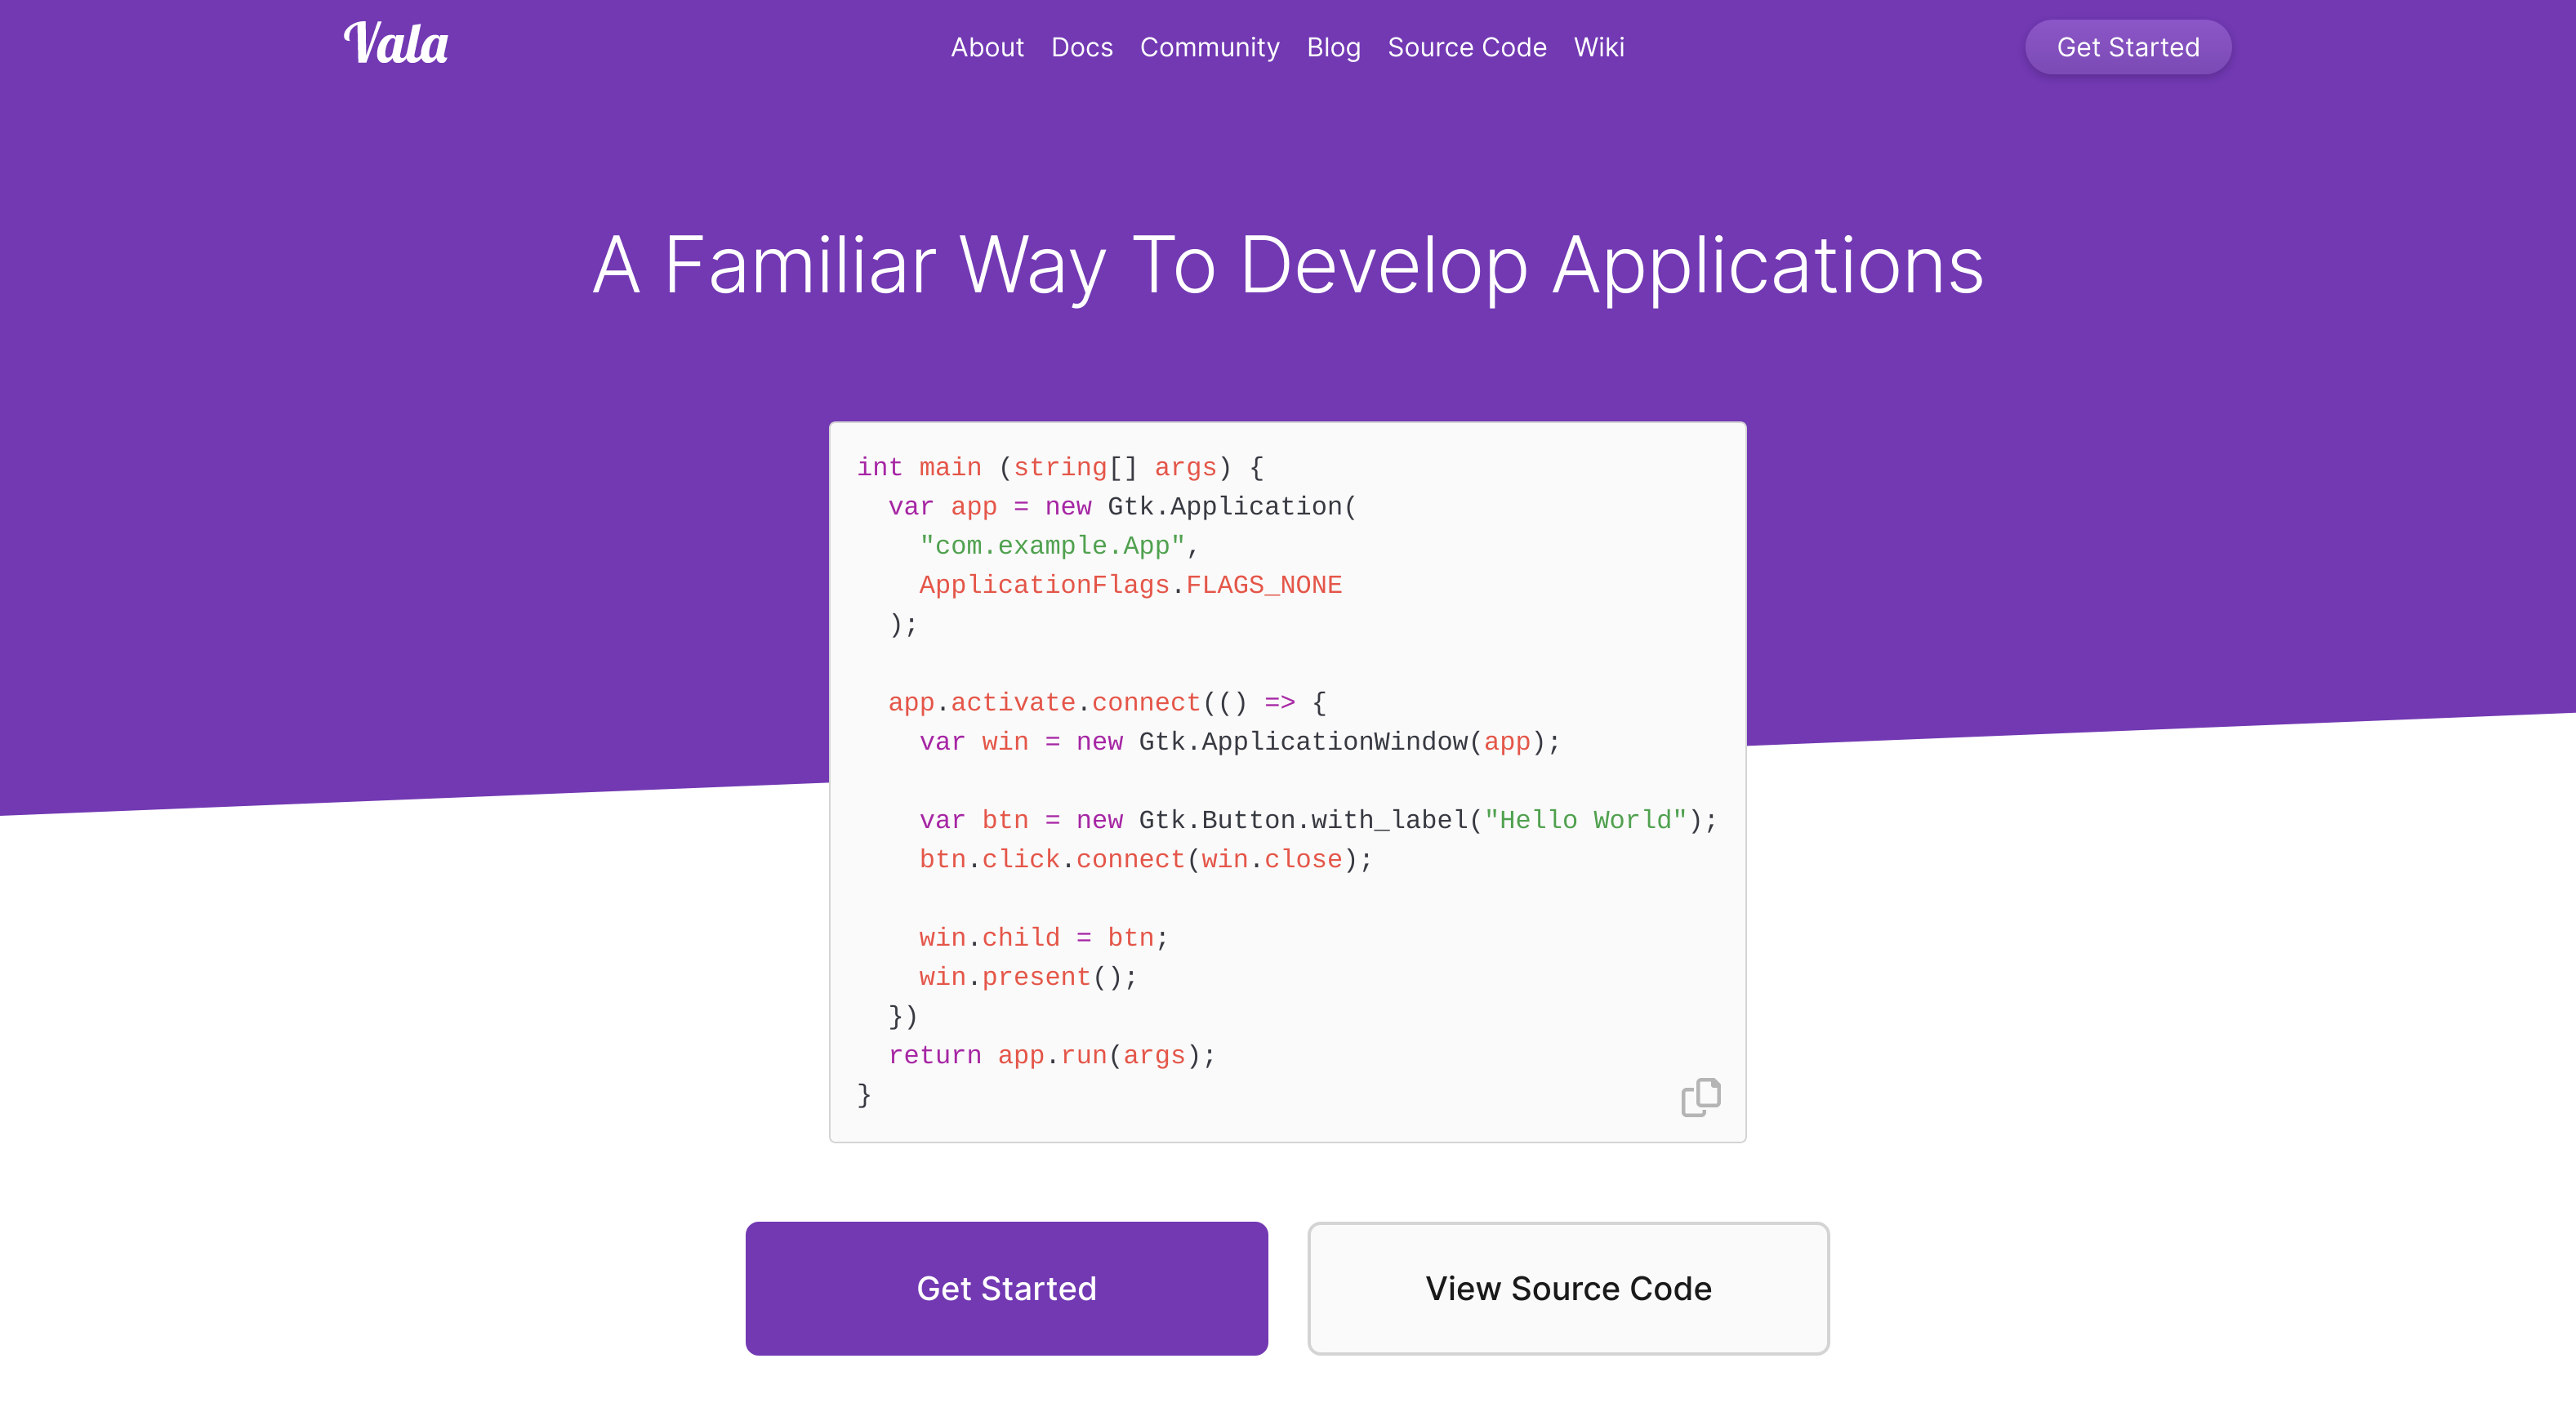
\includegraphics[scale=.09]{res/vala-website.png}
    \end{center}
\end{figure}

{\small WIP: \url{https://github.com/vala-lang/vala-www}}
\end{frame}

\section{Future plans}
\subsection{Static analyzer}
\begin{frame}[c]{Static analyzer}
A static analyzer will help catch bugs and improve code quality.

GCC has \texttt{-fanalyzer}, clang has \texttt{scan-build}.

Work has started on a static analyzer for Vala. Idea is to have this integrated in \texttt{valac} and enabled with \texttt{--analyzer}.

{\small WIP: \url{https://gitlab.gnome.org/Prince781/vala/-/tree/wip/prince781/meson/abstract-interpreter}}
\end{frame}

\begin{frame}[c]{Static analyzer - features}
Current: non-null, arithmetic safety, unreachable code detection, assertion failures
\end{frame}

\begin{frame}[c]{Static analyzer - non-null}
Can detect and prevent all null pointer accesses.

\begin{figure}
    \begin{center}
        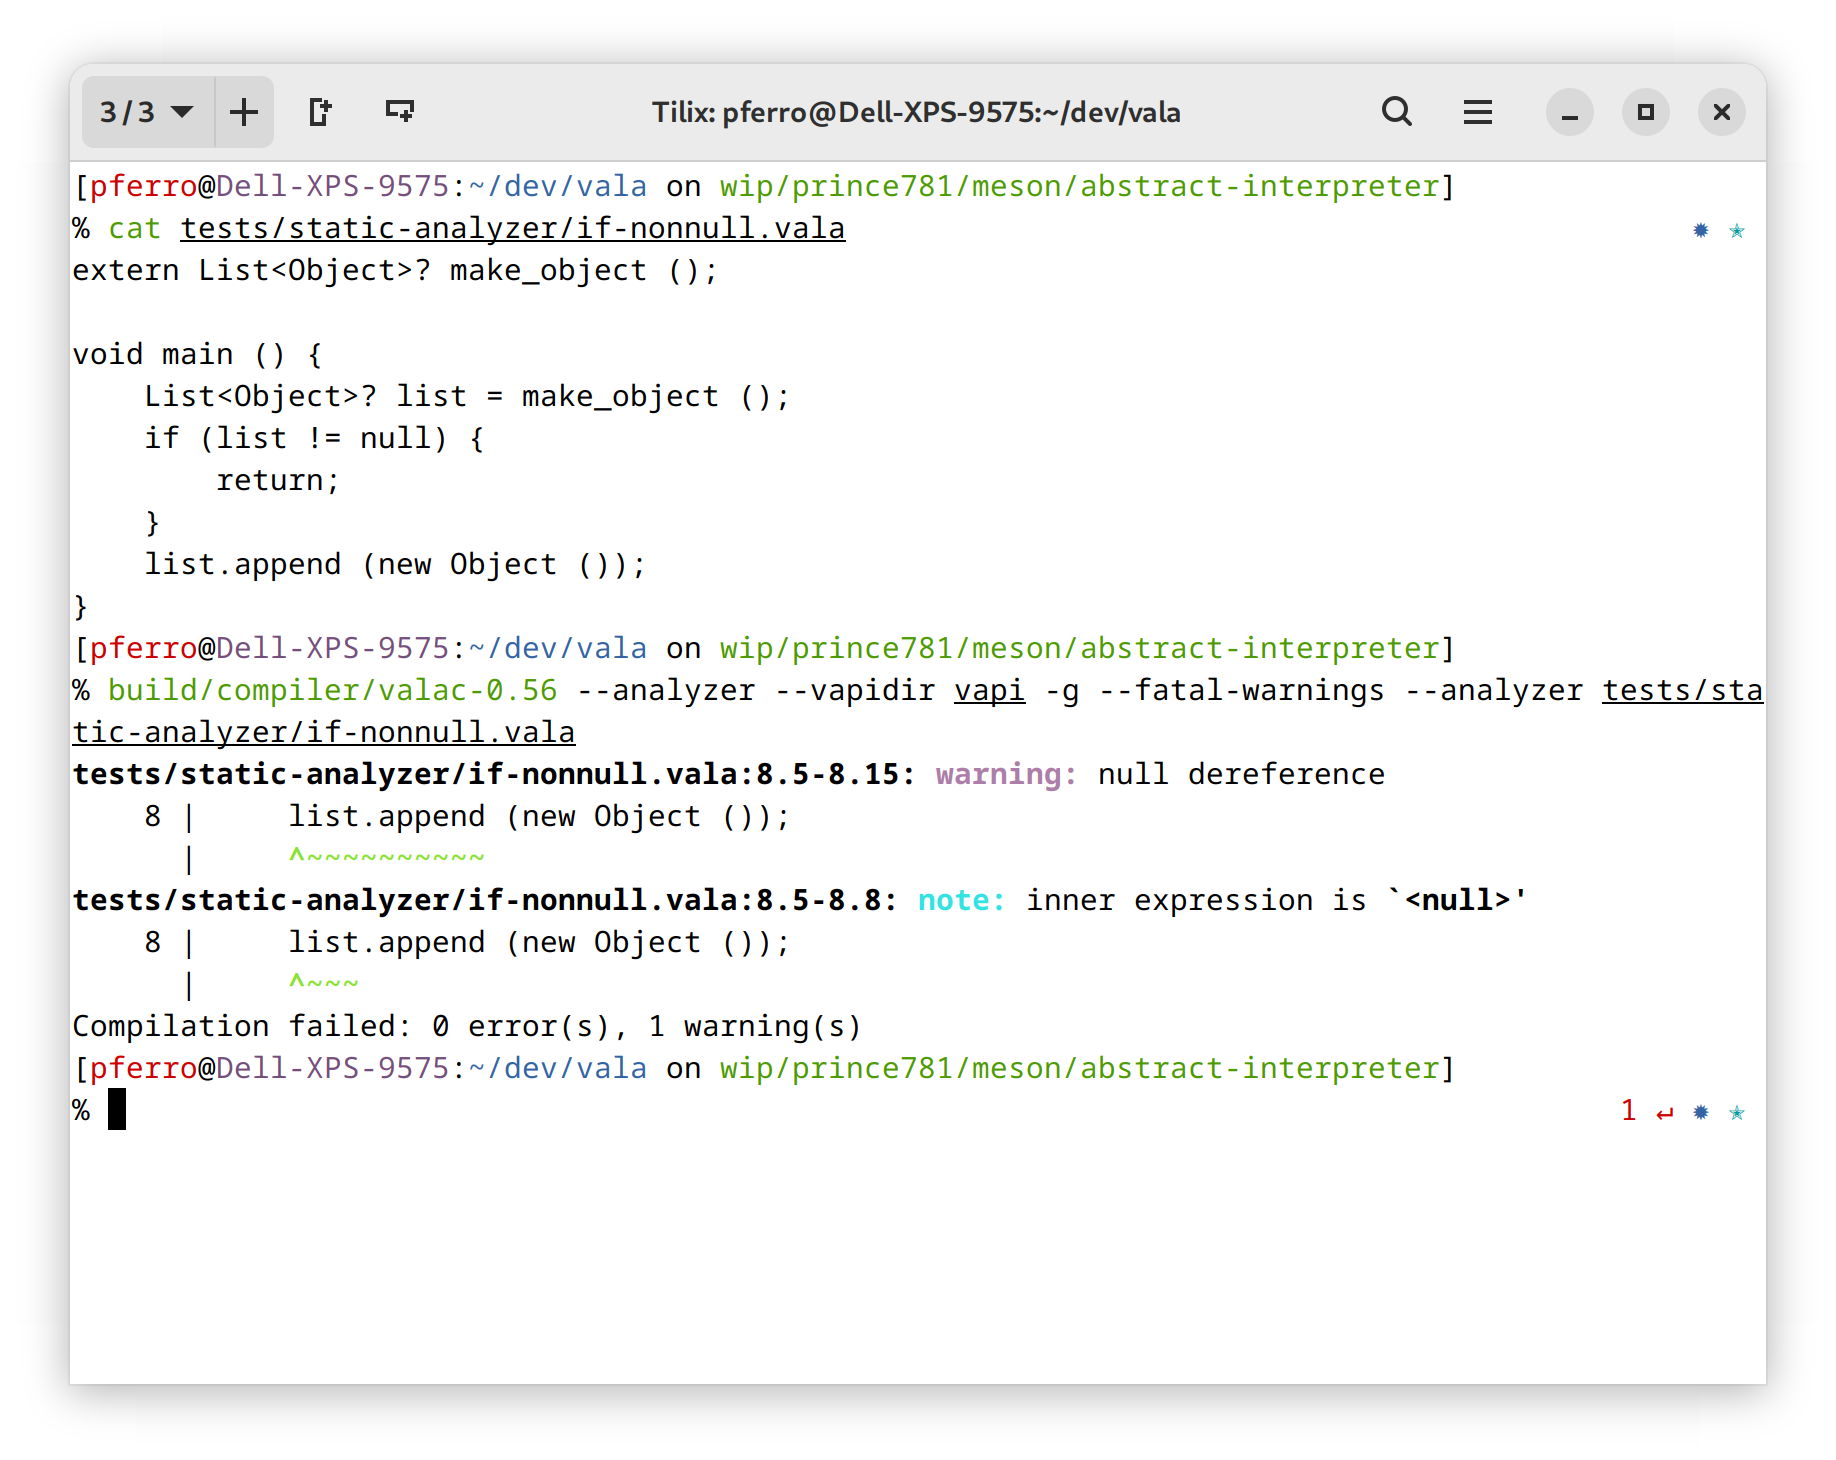
\includegraphics[scale=.12]{res/static-analyzer-nonnull.png}
    \end{center}
\end{figure}
\end{frame}

\begin{frame}[c]{Static analyzer - arithmetic safety}
Can detect and prevent division by zero.

\begin{figure}
    \begin{center}
        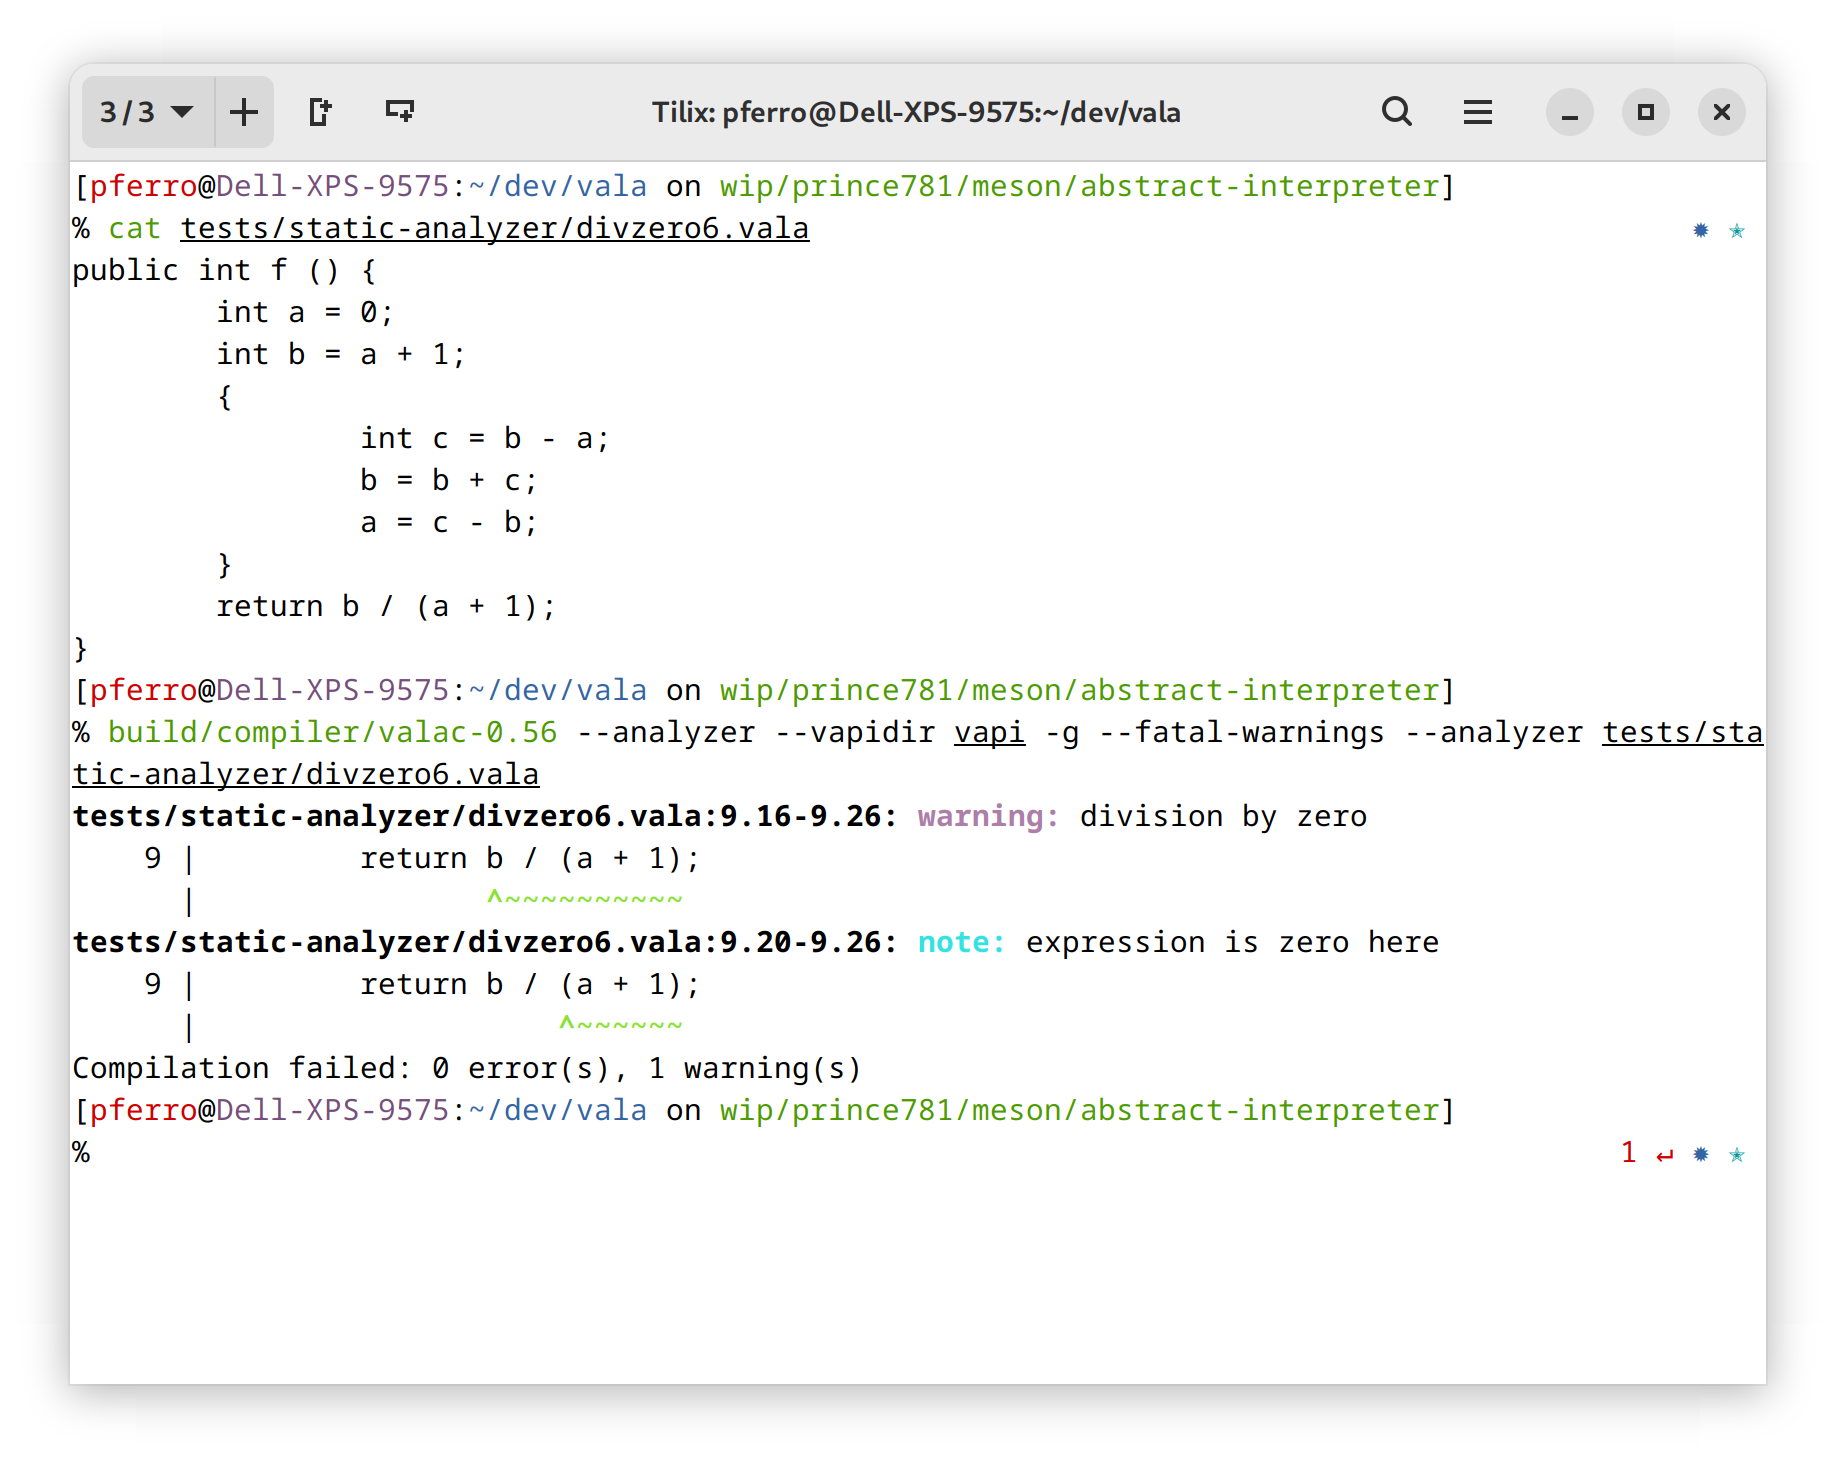
\includegraphics[scale=.12]{res/static-analyzer-divzero.png}
    \end{center}
\end{figure}
\end{frame}

\begin{frame}[c]{Static analyzer - loop nontermination}
Can detect and prevent loop nontermination

\begin{figure}
    \begin{center}
        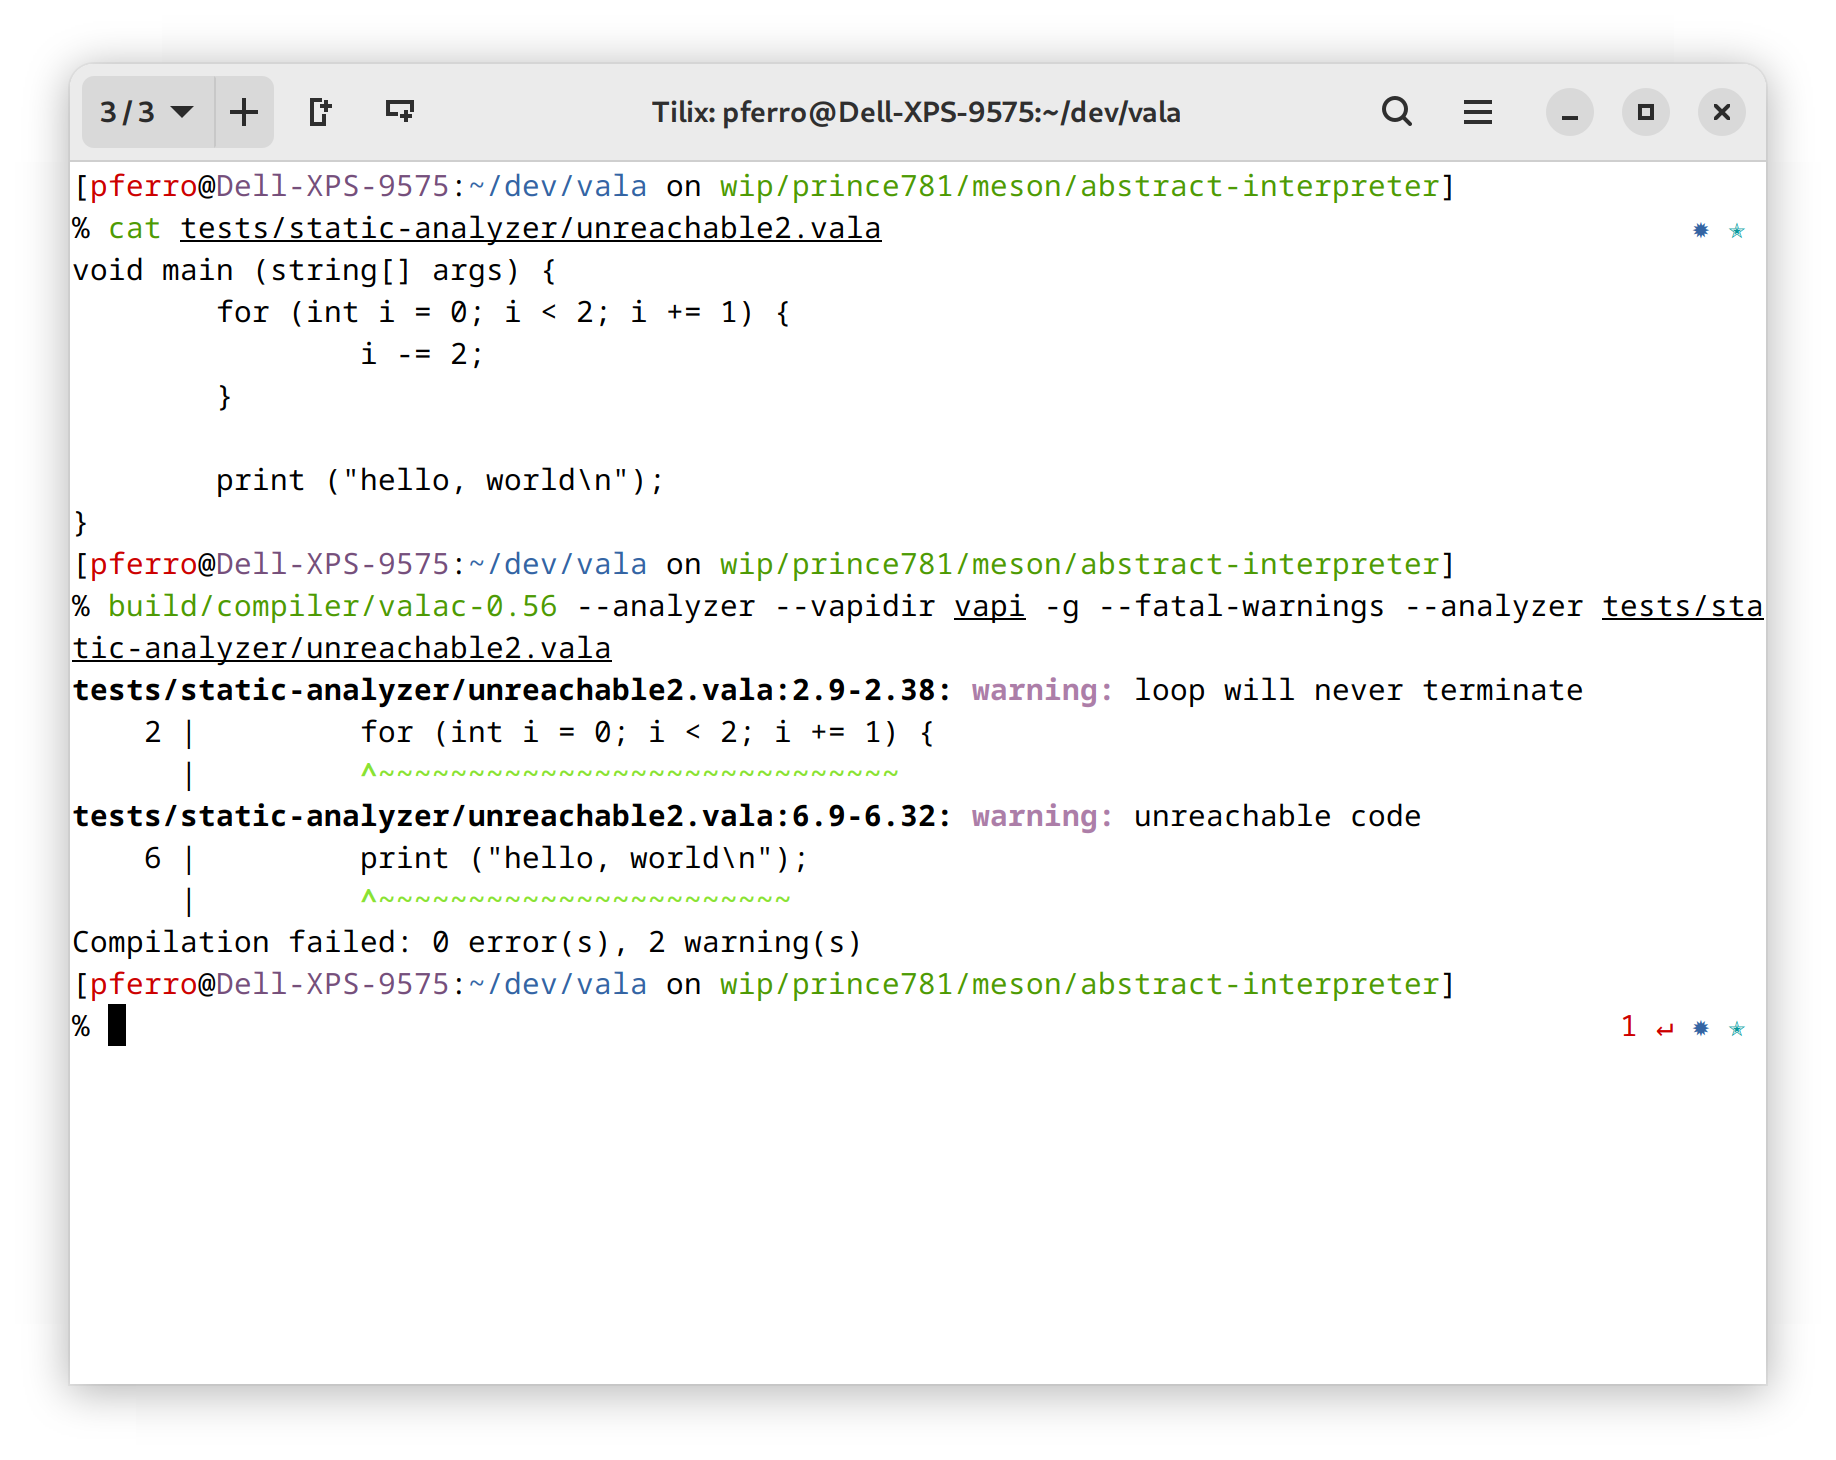
\includegraphics[scale=.12]{res/static-analyzer-loop-nontermination.png}
    \end{center}
\end{figure}
\end{frame}

\subsection{Improving the language}
\begin{frame}[c]{Improving the language}
More expressive language: sum types, type constraints, monomorphization

More safety features: \texttt{unsafe} keyword and default non-null
\end{frame}

\subsection{Debugging}
\begin{frame}[c]{Debugging}
You can use \texttt{gdb} on Vala programs but it's not a fun experience.

Fork GDB and add Vala support?
\begin{itemize}
    \item Hijack expression parser to support Vala syntax
    \item Demangle function names
    \item Display GObject type hierarchy
\end{itemize}
\end{frame}

\subsection{Code actions}
\begin{frame}[c]{Code actions}
Improve the language server with more code actions and quick fixes

Have sophisticated quick fixes, a la Rust's \texttt{clippy}
\end{frame}

\begin{frame}[c]{In closing}
There's been a lot of improvements to Vala development in the last 2 years

If you're interested you can go to \url{https://vala.dev}, check out \texttt{\#vala} on IRC and our \href{https://discord.com/invite/YFAzjSVHt7}{Discord}
\end{frame}

\end{document}